\chapter{Apparent Concavity of the Objective Function for S\&P500 Returns}


%When using the S&P returns, you should find a concave objective function. There is a good reason for that! But it took me a moment to realize... Will you be able to understand why? A straight 6 to each assignment which explains why!

It seems that when using the S\&P500 returns we find a \emph{concave} objective function when using $W=I$, however this is not entirely true: the function is indeed concave on its upper part (it is even asymptotically bounded, but this was also the case for the randomly generated returns !), however in the vicinity of the optimal $\nu$ it is convex. \smallskip
\par
By construction, the possible range we have set for $\nu$ is $\{5;30\}$ with $\nu$ only able to take integer values. The first constraint is due to the expression of the fourth order moment condition $C_1$:
\begin{align*}
    C_1 &= E\left[X^4\right] - \left(\frac{6}{\nu-4}+3\right)\cdot E^2\left[X^2\right] \\
    C_2 &= E\left[X^2\right] - \frac{\nu}{\nu - 2}
\end{align*}
Therefore excluding $\nu = 4$, $C_2$ also excludes $\nu=2$; $3$ is not necessarily excluded, but produces non-optimal values for our data-set.
\smallskip\par
However if we relax the integer constraint on the number of degrees of freedom and treat the objective function as a continuous function instead of the discreet case, we obtain a completely different result !


\section{A Continuous Approach}

\subsection{Local Optimum of the Objective Function}

We now set $\nu \in \; ]4;30]$ and run the exact same analysis as previously (For clarity we restrict the domain to $[4.2;6]$). Results presented in Figure \ref{ConcavitySPI} use the objective function described by $Criterion_I = C^T I C$.
\begin{figure}
    \centering
    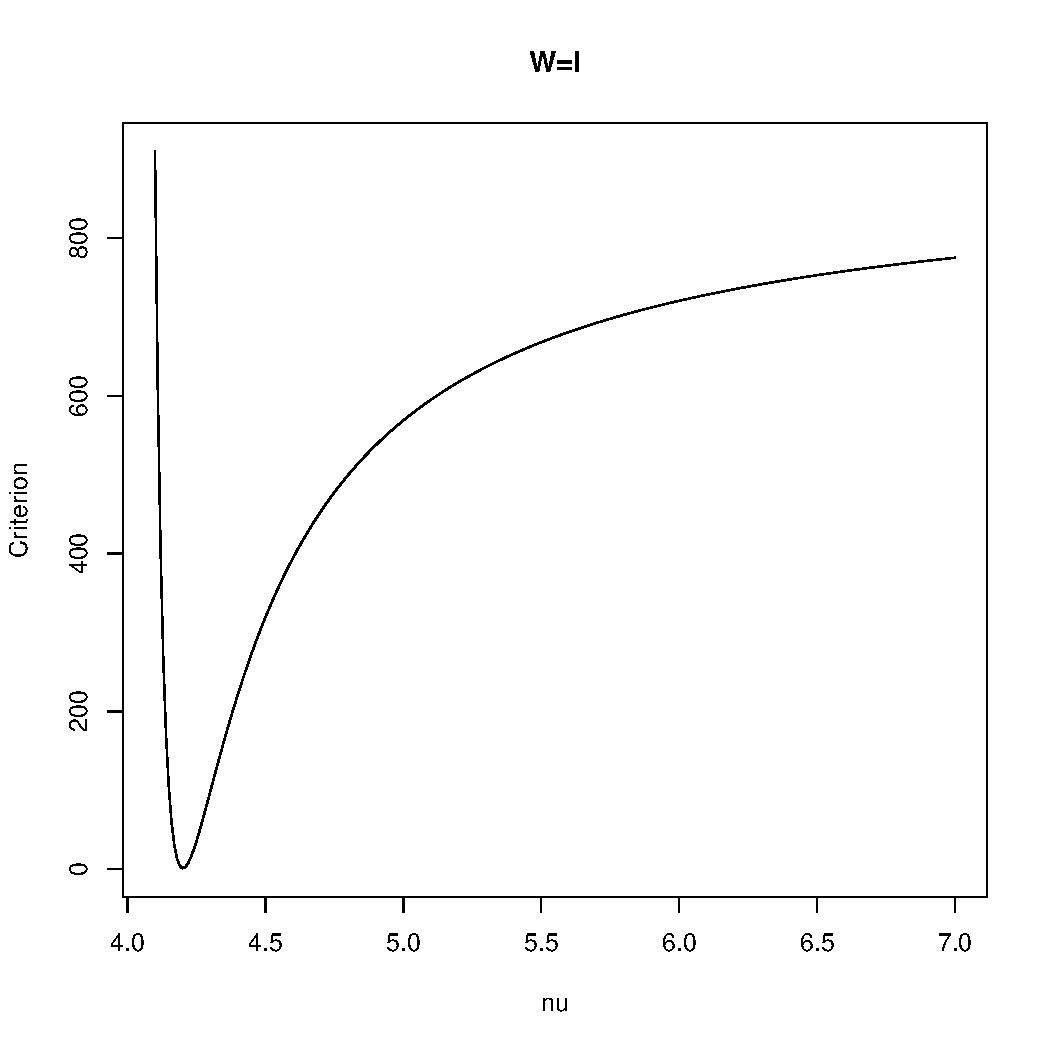
\includegraphics[width=0.95\textwidth]{ConcavityS&PI.pdf}
    \caption{Objective function of the $\nu$ parameter for S\&P500 returns using $W=I$}
    \label{ConcavitySPI}
\end{figure}
\par
Complete fucking game-changer boys ! First of all the function now appears to be convex from $4$ to roughly $4.4$ and only then does it take on a concave appearance. And secondly the objective function seems to be minimised by a unique value of $\nu$ that is not a boundary of domain.
\par
The empirical optimal value for which the $O_f$ is minimised is $\nu=4.2$. 
This can easily be verified by computing the first derivative of the objective function for our specific case:
\begin{equation}\label{ObjectiveFunction_I}
    O_f = \left[E\left[X^4\right] - \left(\frac{6}{\nu-4}+3\right)\cdot         
                E^2\left[X^2\right]\right]^2 +
            \left[E\left[X^2\right] - \frac{\nu}{\nu - 2}\right]^2
\end{equation}

We substitute $E\left[X^4\right]$ and $E\left[X^2\right]$ by their respective empirical approximations for our scaled S\&P500 returns : $32.83457$ and $0.9998292$, this gives us:

\begin{align}\label{FirstDerivativeOf_Of_I}
    \begin{split}
        \pdv{O_f}{\nu} &= \pdv{\nu} \; \left[ \left(32.83457 - (\frac{6}{\nu-4} + 3) \cdot
                            0.9998292^2 \right)^2 + \left(0.9998292 - \frac{\nu}{\nu - 2}\right)^2 \right] \\
                        &= \frac{357.904 \nu^4 - 3658.99 \nu^3 + 13412.2 \nu^2 - 21290 \nu + 12540.5}{(\nu - 4)^3 (\nu - 2)^3}
    \end{split}
\end{align}


Solving $\nu$ for  $\pdv{O_f}{\nu}=0$ gives two solutions: $\nu_1^* \approx 2.37458$ and $\nu_2^* \approx 4.20105$, we can disregard $\nu_1$ as it is not part of the set domain (Furthermore $O_f(\nu_1) > O_f(\nu_2)$), however $\nu_2^*$ \emph{is} part of our domain and is not one of the boundaries. \smallskip
\par
Therefore implying the optimal value of $\nu$ to fit our distribution of scaled S\&P500 returns is $4.20105$ which is consistent with the value found previously.

\subsection{Local Convexity \& Concavity of the $O_f$}

After having addressed the question of the "true" local minimum of the function, we now turn to the apparent concavity of the $O_f$ as presented in Figure \ref{SP500_returns_criterion} when using $W=I$ \bigskip\par
Using the objective function described by Equation \ref{ObjectiveFunction_I} and the empirical values used to compute the first derivative (Equation \ref{FirstDerivativeOf_Of_I}) we can also derive the second derivative of the $O_f$ :
\begin{equation}\label{SecondDerivativeOf_Of_I}
    \pdv[2]{O_f}{\nu} =  \frac{-715.808 \nu^5 + 8829.54 \nu^4 - 42196 \nu^3 + 99107.5 \nu^2 - 116127 \nu + 55408.8}{(\nu - 4)^4 (\nu - 2)^4}
\end{equation}

If we solve for $\pdv[2]{O_f}{\nu} = 0$ we obtain a single real root: $\nu^{**} \approx 4.30156$ indicating a point of inflexion of the $O_f$ at $\nu^{**}$ 
\smallskip \par
In addition, let $O_f^{''}=\pdv[2]{O_f}{\nu}$ , results for $\nu \in \; [2;5.5]$ are shown in Figure \ref{SecondDerivativePlot_I}:
\begin{equation*}
    \begin{cases}
        O_f^{''} > 0 \; , \; \nu \in \; ]-\infty;2[ \\
        O_f^{''} \text{ undefined } \; , \; \nu = 2 \\
        O_f^{''} > 0 \; , \; \nu \in \; ]2;4[ \\
        O_f^{''} \text{ undefined } \; , \; \nu = 4 \\
        O_f^{''} > 0 \; , \; \nu \in \; ]4;\nu^{**}[ \\
        O_f^{''} = 0 \; , \; \nu = \nu^{**} \\
        O_f^{''} < 0 \; , \; \nu \in \; ]\nu^{**};\infty[ \\
    \end{cases}
\end{equation*}

Therefore the $O_f$ is convex between $4$ and $\nu^{**} \approx 4.30156$ so the local minimum of the function calculated in (\ref{FirstDerivativeOf_Of_I}) is situated on the convex portion.
\smallskip\par
In contrast, from $\nu^{**} \approx 4.30156$ to $\infty$ the $O_f$ is strictly concave which is why it appeared concave in Figure \ref{SP500_returns_criterion} since the range used was $\{5:30\}$

\section{Generalisation and Further Development}

The previous analysis can be generalised to the case where the objective function is such that (cf. Figure \ref{ConcavitySPW}):
\begin{equation*}
    O_f = C^T \Sigma^{-1} C \; \; \; ; \; \;
        \Sigma=
    \begin{bmatrix}[c]
        \sigma_{m_1,m_1}    & \sigma_{m_1,m_2} \\
        \sigma_{m_2,m_1}    & \sigma_{m_2,m_2}
    \end{bmatrix}
    \;\; ; \; \; C = 
    \begin{bmatrix}[l]
        E[X^4]-E[X^2]^2(\frac{6}{\nu-4}+3)  \\
        E[X^2]-\frac{\nu}{\nu-2}
    \end{bmatrix}
\end{equation*}
In fact this was also the case for the randomly generated t-returns in the first part of Exercise 1, the functions represented in Figure \ref{t-returns_criterion} are not strictly convex, they are also concave on the upper part of the function.
\begin{figure}
    \centering
    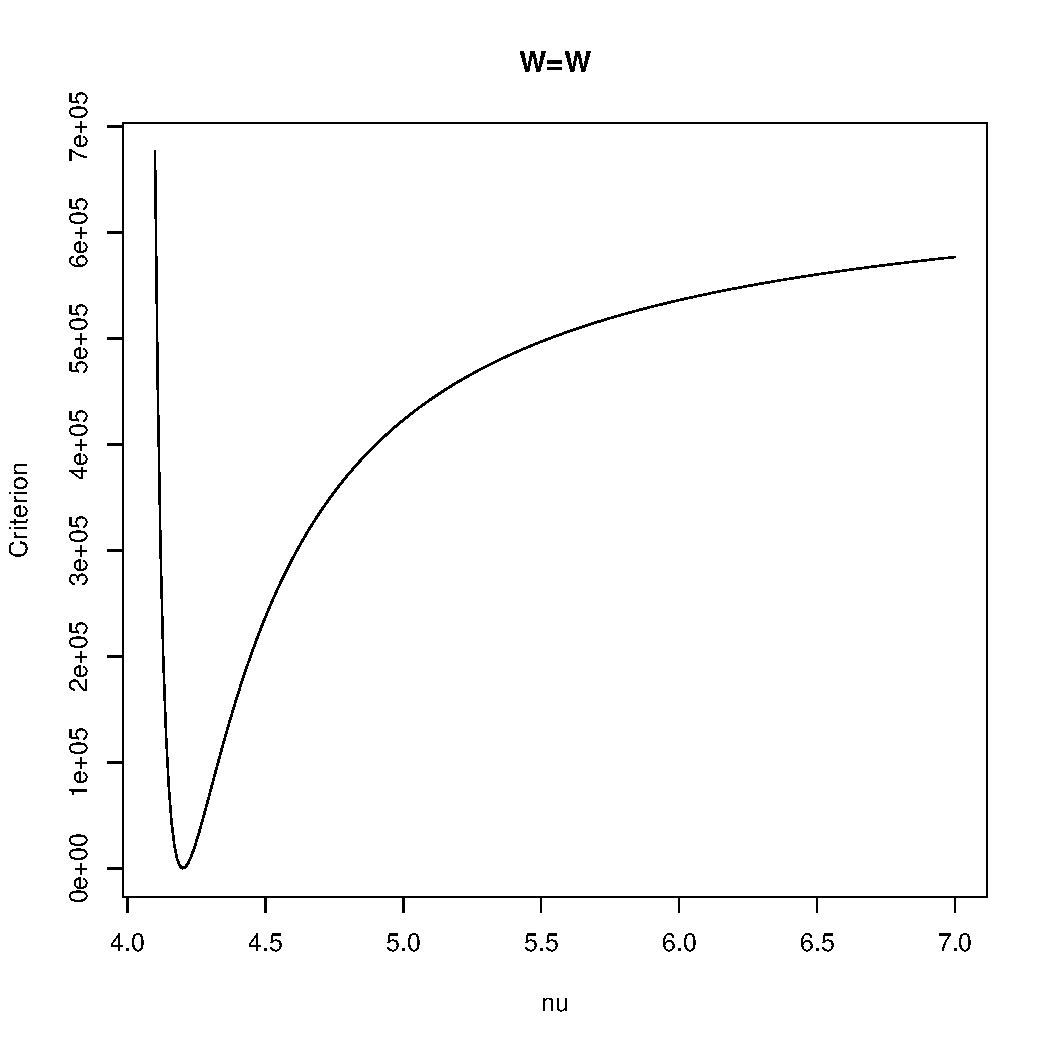
\includegraphics[width=0.6\textwidth]{ConcavityS&PW.pdf}
    \caption{Objective function of $\nu$ parameter for S\&P500 returns using $W=\Sigma^{-1}$}
    \label{ConcavitySPW}
\end{figure}
This can be demonstrated by the fact that the second derivative of the objective function for our randomly generated t-returns is negative after $\nu^*$.
\smallskip\par
Intuitively this can be seen by calculating the limit of the $O_f$ when $\nu$ tends to infinity, this limit exists and is finite, however it is unique to each data-set (provided each data-set is different): it is the value of the objective function that measures the distance between the data-set and the Normal Distribution. In the case of our S\&P500 returns when using $Criterion_I$ :
\begin{equation*}
    \lim_{\nu \to \infty}O_f = \lim_{\nu \to \infty}C^T I C = 890.163
\end{equation*}

\subsection{Non-Integer Degrees of Freedom}
The initial issue arose from the fact that we use the number of degrees of freedom as one of the inputs for the object; however the degrees of freedom can theoretically only take integer values.
\smallskip\par
When allowing $\nu$ to take non-integer values we "denature" the idea of a degree of freedom. There is some literature concerning non-integer values for degrees of freedom: indeed in a few circumstances you can establish that the degrees of freedom to fit the data for some particular models must be between some value $k$ and $k+1$.
\smallskip\par
We usually think of degrees of freedom as the number of free parameters, but there are situations where the parameters are not completely free and they can then be difficult to count. This can happen when smoothing / regularizing, for example. This could possibly refer to the Welch–Satterthwaite equation.